% !TEX TS-program = lualatex
% !TEX encoding = UTF-8 Unicode

\documentclass[12pt, letterpaper]{article}

%%BIBLIOGRAPHY- This uses biber/biblatex to generate bibliographies according to the 
%%Unified Style Sheet for Linguistics
\usepackage[main=american, german]{babel}% Recommended
\usepackage{csquotes}% Recommended
\usepackage[backend=biber,
             style=unified,
             maxcitenames=3,
             maxbibnames=99,
             natbib,
             url=false]{biblatex}
\addbibresource{Library.bib}
\setcounter{biburlnumpenalty}{100}  % allow URL breaks at numbers
%\setcounter{biburlucpenalty}{100}   % allow URL breaks at uppercase letters
%\setcounter{biburllcpenalty}{100}   % allow URL breaks at lowercase letters

%%TYPOLOGY
\usepackage[svgnames]{xcolor} % Specify colors by their 'svgnames', for a full list of all colors available see here: http://www.latextemplates.com/svgnames-colors
%\usepackage[compact]{titlesec}
%\titleformat{\section}[runin]{\normalfont\bfseries}{\thesection.}{.5em}{}[.]
%\titleformat{\subsection}[runin]{\normalfont\scshape}{\thesubsection}{.5em}{}[.]
\usepackage[hmargin=1in,vmargin=1in]{geometry}  %Margins
\usepackage{graphicx} % 
\usepackage{stackengine} %Package to allow text above or below other text, Also helpful for HG weights 
\usepackage{fontspec} %Selection of fonts must be ran in XeLaTeX
\usepackage{amssymb} %Math symbols
\usepackage{amsmath} % Mathematical enhancements for LaTeX
\usepackage{setspace} %Linespacing
\usepackage{multicol} %Multicolumn text
\usepackage{enumitem} %Allows for continuous numbering of lists over examples, etc.
\usepackage{multirow} %Useful for combining cells in tablesbrew 
\usepackage{booktabs}
\usepackage{hanging}
\usepackage{fancyhdr} %Allows for the 
\pagestyle{fancy}
\fancyhead[L]{\textit{QP Defense Handout}} 
\fancyhead[R]{\textit{\today}} 
\fancyfoot[L,R]{} 
\fancyfoot[C]{\thepage} 
\renewcommand{\headrulewidth}{0.4pt}
\setlength{\headheight}{14.5pt} % ...at least 14.49998pt
% \usepackage{fourier} % This allows for the use of certain wingdings like bombs, frowns, etc.
% \usepackage{fourier-orns} %More useful symbols like bombs and jolly-roger, mostly for OT
\usepackage[colorlinks,allcolors={black},urlcolor={blue}]{hyperref} %allows for hyperlinks and pdf bookmarks
% \usepackage{url} %allows for urls
% \def\UrlBreaks{\do\/\do-} %allows for urls to be broken up
\usepackage[normalem]{ulem} %strike out text. Handy for syntax
\usepackage{tcolorbox}
\usepackage{datetime2}
\usepackage{caption}
\usepackage{subcaption}

%%FONTS
\setmainfont{Libertinus Serif}
\setsansfont{Libertinus Sans}
\setmonofont[Scale=MatchLowercase]{Libertinus Mono}

%%PACKAGES FOR LINGUISTICS
%\usepackage{OTtablx} %Generating tableaux with using TIPA
\usepackage[noipa]{OTtablx} % Use this one generating tableaux without using TIPA
%\usepackage[notipa]{ot-tableau} % Another tableau drawing packing use for posters.
% \usepackage{linguex} % Linguistic examples
% \usepackage{langsci-linguex} % Linguistic examples
\usepackage{langsci-gb4e} % Language Science Press' modification of gb4e
% \usepackage{langsci-avm} % Language Science Press' AVM package
\usepackage{tikz} % Drawing Hasse diagrams
% \usepackage{pst-asr} % Drawing autosegmental features
\usepackage{pstricks} % required for pst-asr, OTtablx, pst-jtree.
% \usepackage{pst-jtree} %Syntax tree draawing software
% \usepackage{tikz-qtree} % Another syntax tree drawing software. Uses bracket notation.
\usepackage[linguistics]{forest} % Another syntax tree drawing software. Uses bracket notation.
% \usepackage{ling-macros} % Various linguistic macros. Does not work with linguex.
% \usepackage{covington} % Another linguistic examples package.
\usepackage{leipzig} % Offers support for Leipzig Glossing Rules

%%LEIPZIG GLOSSING FOR ZAPOTEC
\newleipzig{el}{el}{elder} % Elder pronouns
\newleipzig{hu}{hu}{human} % Human pronouns
\newleipzig{an}{an}{animate} % Animate pronouns
\newleipzig{in}{in}{inanimate} % Inanimate pronouns
\newleipzig{pot}{pot}{potential} % Potential Aspect
\newleipzig{cont}{cont}{continuative} % Continuative Aspect
% \newleipzig{pot}{pot}{potential} % Potential Aspect
\newleipzig{stat}{stat}{stative} % Potential Aspect
\newleipzig{and}{and}{andative} % Andative Aspect
\newleipzig{ven}{ven}{venative} % Venative Aspect
% \newleipzig{res}{res}{restitutive} % Restitutive Aspect
\newleipzig{rep}{rep}{repetitive} % Repetitive Aspect

%%TITLE INFORMATION
\title{TITLE}
\author{Mykel Loren Brinkerhoff}
\date{\today}

%%MACROS
\newcommand{\sub}[1]{\textsubscript{#1}}
\newcommand{\supr}[1]{\textsuperscript{#1}}
\providecommand{\lsptoprule}{\midrule\toprule}
\providecommand{\lspbottomrule}{\bottomrule\midrule}
\newcommand{\fittable}[1]{\resizebox{\textwidth}{!}{#1}}

\makeatletter
\renewcommand{\paragraph}{%
  \@startsection{paragraph}{4}%
  {\z@}{0ex \@plus 1ex \@minus .2ex}{-1em}%
  {\normalfont\normalsize\bfseries}%
}
\makeatother
\parindent=10pt


\begin{document}

%%If using linguex, need the following commands to get correct LSA style spacing
%% these have to be after  \begin{document}
    % \setlength{\Extopsep}{6pt}
    % \setlength{\Exlabelsep}{9pt}%effect of 0.4in indent from left text edge
%%

%% Line spacing setting. Comment out the line spacing you do not need. Comment out all if you want single spacing.
%\doublespacing
%\onehalfspacing

\begin{center}
    {\Large \textbf{The acoustics of phonation in Santiago Laxopa Zapotec}}
    \vspace{6pt}

    Mykel Loren Brinkerhoff
\end{center}
%\maketitle
%\maketitleinst
\thispagestyle{fancy}

\tableofcontents

%------------------------------------
\section{Introduction} \label{sec:Introduction}
%------------------------------------

\begin{itemize}
    \item 
\end{itemize}

%------------------------------------
\section{Background} \label{sec:Background}
%------------------------------------


%------------------------------------
\section{Santiago Laxopa Zapotec} \label{sec:SLZ}
%------------------------------------

\begin{itemize}
    \item Santiago Laxopa Zapotec (SLZ), endonym \textit{Dille'xhunh Laxup}, is a a Northern Zapotec language spoken by approximately 1000 people in the municipality of Santiago Laxopa, Ixtlán, Oaxaca, Mexico and in diaspora communities in Mexico and the United States \citep{adlerAcousticsPhonationTypes2016,adlerDerivationVerbInitiality2018,foleyForbiddenCliticClusters2018,foleyExtendingPersonCaseConstraint2020}.
    \item Closely related to San Bartolomé Zoogocho Zapotec \citep{longDiccionarioZapotecoSan2005,sonnenscheinDescriptiveGrammarSan2005} and shares a high level of mutual intelligibility with it.
    \item SLZ is similar to other Zapotecan languages in distinguishing lenis and fortis consonants \citep[e.g.,][]{nellisFortisLenisCajonos1980,jaegerFortisLenisQuestion1983,uchiharaFortisLenisGlides2016}.
\end{itemize}

\begin{table}[!h]
	\centering
	\caption{Consonant inventory for Santiago Laxopa Zapotec}
	\label{tab:SLZcons}
	\fittable{
	\begin{tabular}{llcccccccc}
	\lsptoprule
		  &  & bilabial & alveolar  & post- & retroflex & palatal &velar &labio-  &  uvular \\
		 &&&&alveolar&  &&&velar& \\
	\midrule
	stop 		& lenis   & b  & d  & & & & g & gʷ & \\
				& fortis  & p  & t  & & & & k & kʷ & \\
	fricative   & lenis   &    & z  & ʒ & ʐ &  & &  & ʁ \\
		        & fortis  &    & s  & ʃ & ʂ & ç & & & \\
	affricate 	& lenis   &    & d͡z & & & & & & \\
				& fortis  &    & t͡s & & t͡ʃ & & & & \\
    nasal    	& lenis   &	   & n  & & & & & & \\
				& fortis  &	mː & nː & & & & & & \\
	lateral  	& lenis   &    & l & & & & & & \\
				& fortis  &    & lː & & & & & & \\
	trill		& 		  &    & r & & &  & &  & \\ 			
	approximate & 		  &    & & & & & & w & \\ 
	\lspbottomrule
	\end{tabular}
	}
\end{table}

\begin{itemize}
    \item SLZ has a standard five vowel inventory. 
\end{itemize}

\begin{table}[!h]
	\centering
	\caption{Vowel qualities in Santiago Laxopa Zapotec.}
    \label{tab:SLZvowels}
	\begin{tabular}{lccc}
	\lsptoprule
	&  front& central  & back \\
	\midrule
	high   	&  i  &     &   u \\
	mid    	&  e  &   	& 	o \\
	low   	&     &  a 	&	  \\
	\lspbottomrule
	\end{tabular}
\end{table}

\begin{itemize}
	\item These five vowels, additionally, appear with one of four different phonation types which will be discussed in greater detail in Section~\ref{sec:Phonation}.
\end{itemize}

%------------------------------------
\subsection{Tone in Santiago Laxopa Zapotec} \label{sec:Tone}
%------------------------------------

\begin{itemize}
    \item Similar to other Otomanguean languages, SLZ is tonal\citep{suarezMesoamericanIndianLanguages1983,campbellMesoAmericaLinguisticArea1986,silvermanLaryngealComplexityOtomanguean1997,campbellOtomangueanHistoricalLinguistics2017a,campbellOtomangueanHistoricalLinguistics2017}.
    \item SLZ has five distinct tonal patterns that appear on the syllables of nouns, see Table~\ref{tab:tones}. 
\end{itemize}

\begin{table}[!h]
	\centering
	\caption{Examples of the five tonal patterns observed in the Santiago Laxopa Zapotec words.}
	\label{tab:tones}
	\begin{tabular}{lllll}
	\lsptoprule
	High   	&  a\supr{H}  &  \textit{xha}   &  [ ʐa\supr{H} ] & `clothing.\textsc{poss}'\\
	Mid    	&  a\supr{M}  &  \textit{lhill} 	& [ liʒ\supr{M} ] & `house.\textsc{poss}' \\
	Low   	&  a\supr{L}  &  \textit{yu'} 	&	 [ çuˀ\supr{L} ] & `earth'\\
	Rising	&  a\supr{MH}  &  \textit{yu'u} 	&	[ çuˀu\supr{MH} ] & `quicklime (Sp. cal)' \\
	Falling &  a\supr{HL}  &  \textit{yu'u}  &	[çuˀu\supr{HL}] &	`house' \\
	\lspbottomrule
	\end{tabular}
\end{table}

\begin{itemize}
	\item These five tonal patterns are illustrated in Figures~\ref{fig:FSRTonePlot} and \ref{fig:RDTonePlot} for two different SLZ speakers. 
	\item Figures~\ref{fig:FSRTonePlot} and \ref{fig:RDTonePlot} shows the five tonal contrasts averaged for each tonal contrast from the onset to ending of the vowel. 
	\item We can ignore the first 20-25\% of the measure due to the influence of transitions out of the consonantal onsets. 
\end{itemize}

\begin{figure}[!ht]
	\centering
	\includegraphics[width=0.9\textwidth]{../FSRTonePlot.png}
	\label{fig:FSRTonePlot}
	\caption{Tonal contrasts for FSR averaged and time normalized. Each line in this graph represents the average of approximately 10 syllables for each tonal pattern. }
\end{figure}

\begin{figure}[!ht]
	\centering
	\includegraphics[width=0.9\textwidth]{../RDTonePlot.png}
	\label{fig:RDTonePlot}
	\caption{Tonal contrasts for RD averaged and time normalized. Each line in this graph represents the average of approximately 10 syllables for each tonal pattern.}
\end{figure}
%------------------------------------
\subsection{Phonation in Santiago Laxopa Zapotec} \label{sec:Phonation}
%------------------------------------

\begin{itemize}
	\item Zapotecan languages commonly make use of contrastive phonation on vowels \citep[e.g.,][]{avelinobecerraTopicsYalalagZapotec2004,longDiccionarioZapotecoSan2005,avelinoAcousticElectroglottographicAnalyses2010,lopeznicolasEstudiosFonologiaGramatica2016,chavez-peonInteractionMetricalStructure2010}.
	\item SLZ is no different and has four contrastive phonation types: modal /a/, breathy /a̤/, checked /aˀ/, and laryngealized /aˀa/. 
	\item 
\end{itemize}

\begin{figure}[!h]
	\centering
	\begin{subfigure}{.5\textwidth}
		\centering
		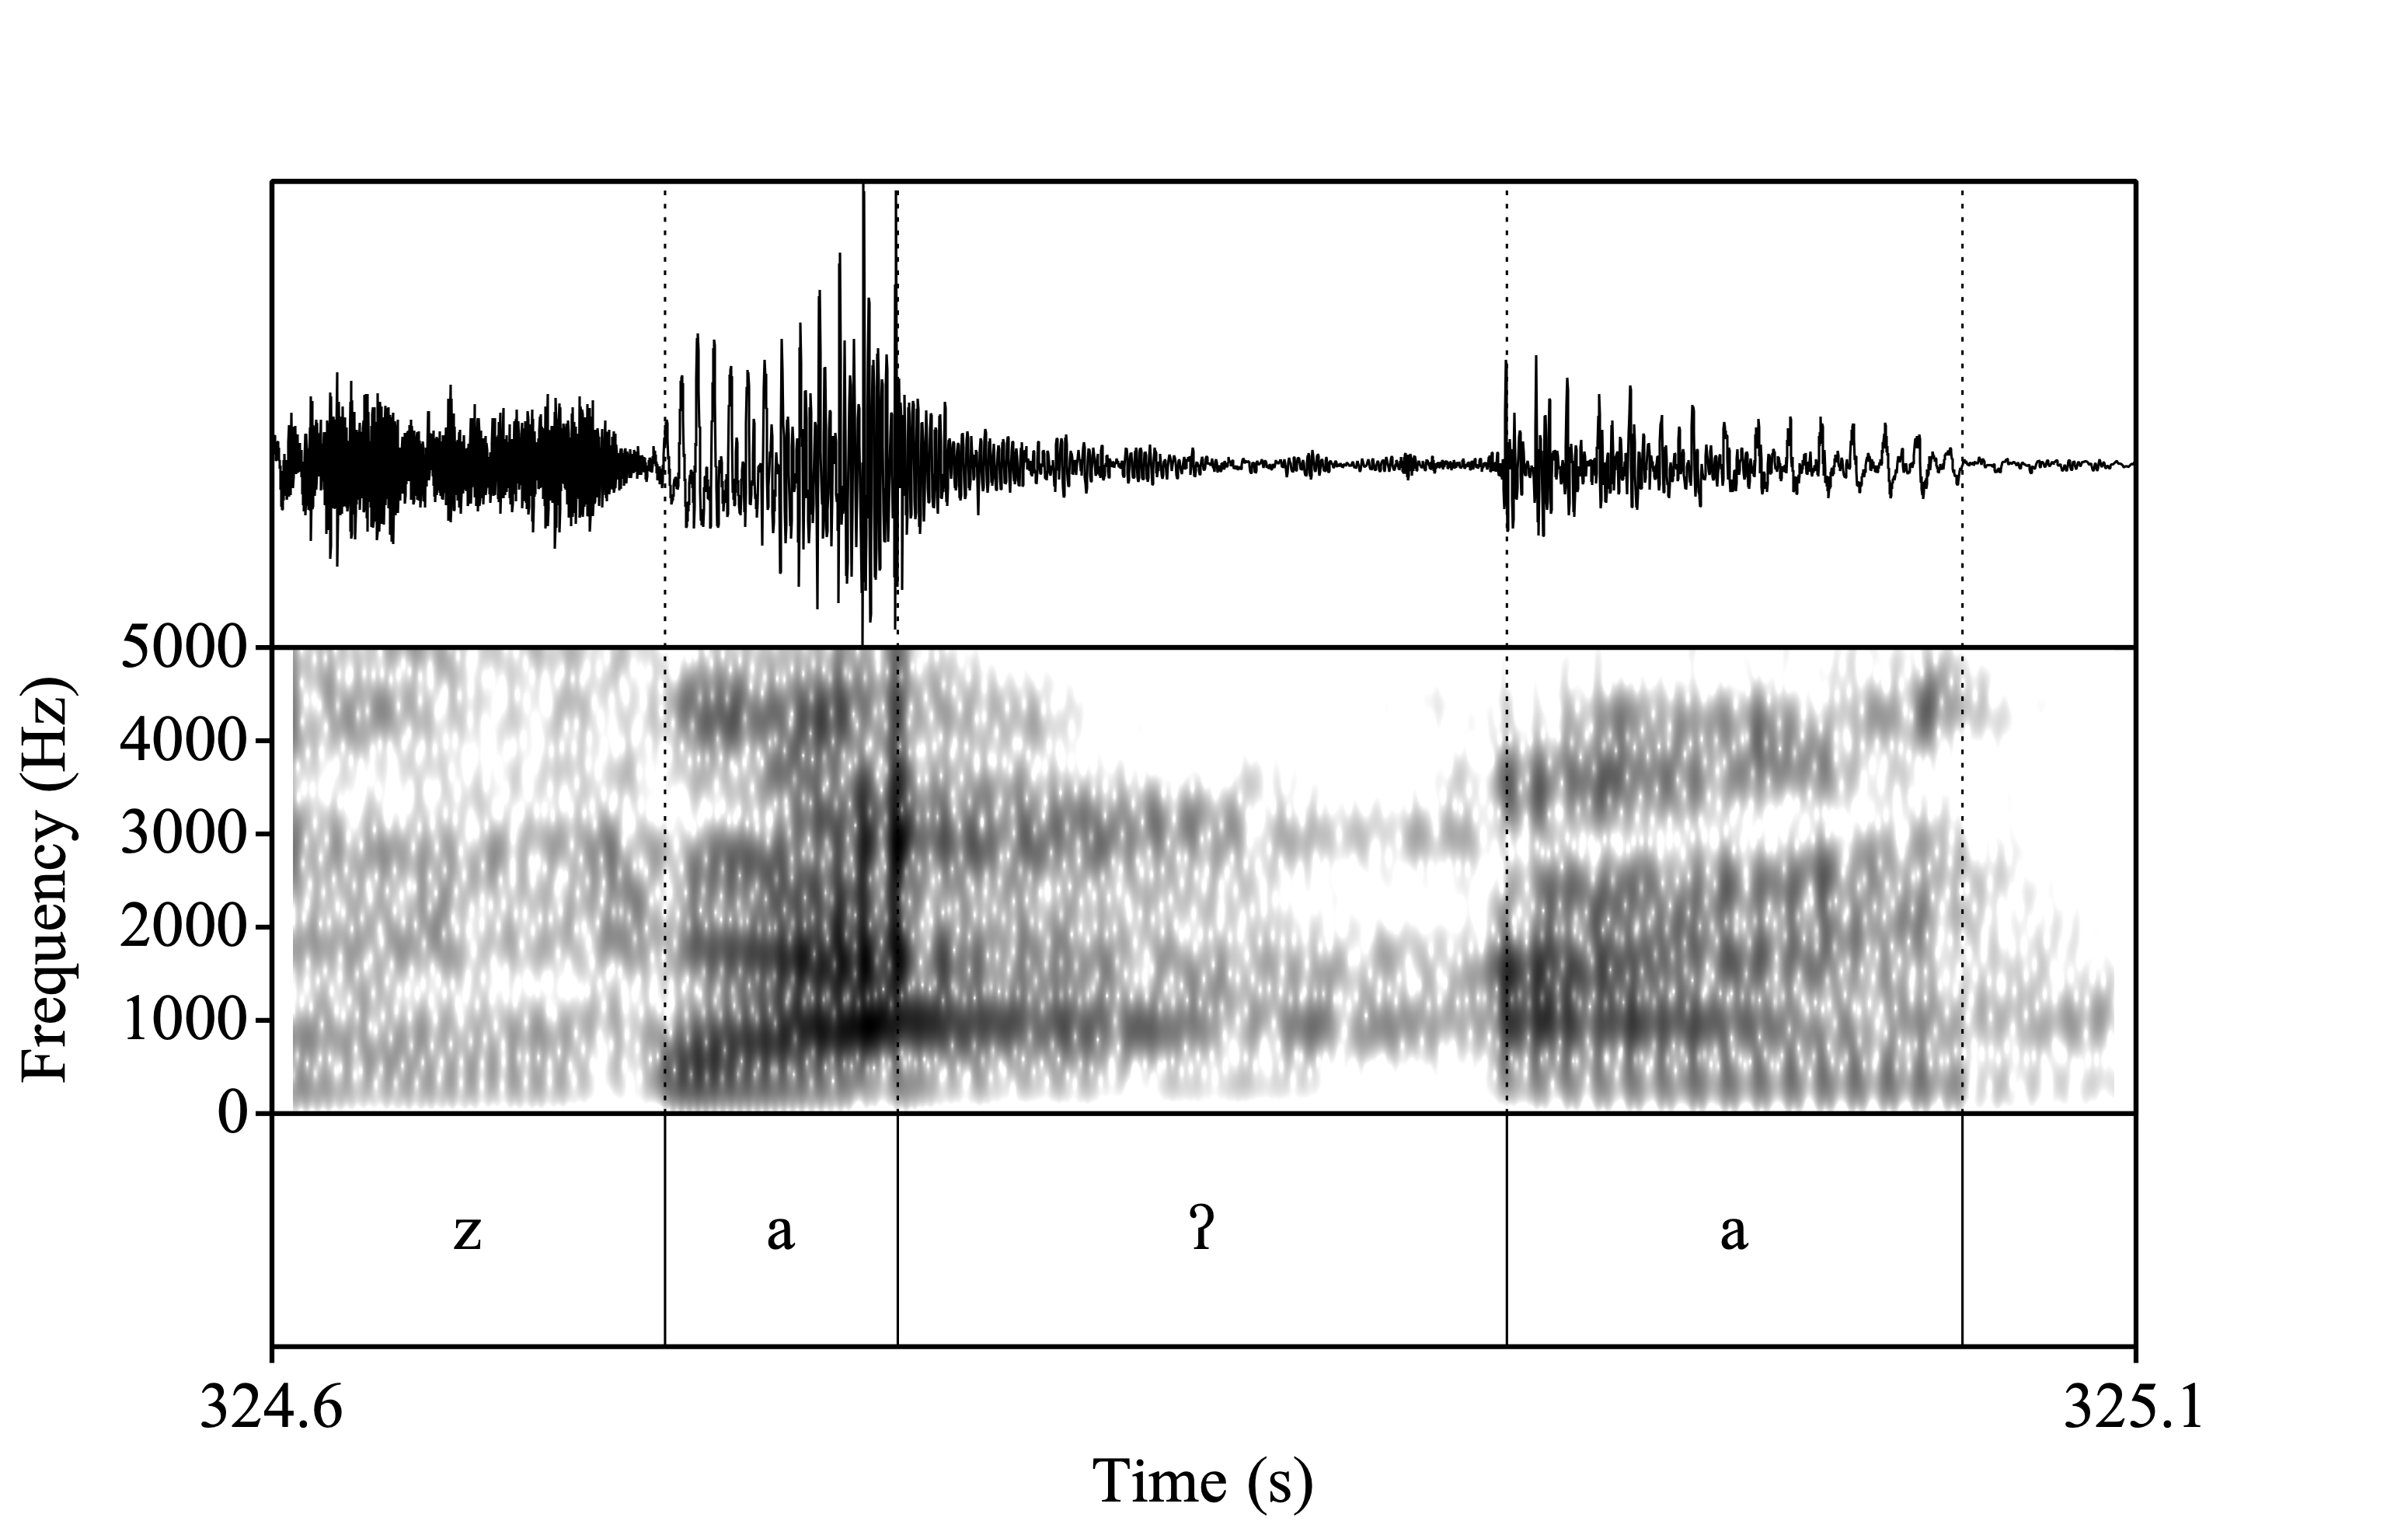
\includegraphics[width=\linewidth]{../za'a.png}
		\caption{\textit{za'a} `corncob'}
		\label{fig:za'a}
	\end{subfigure}%
	\begin{subfigure}{.5\textwidth}
		\centering
		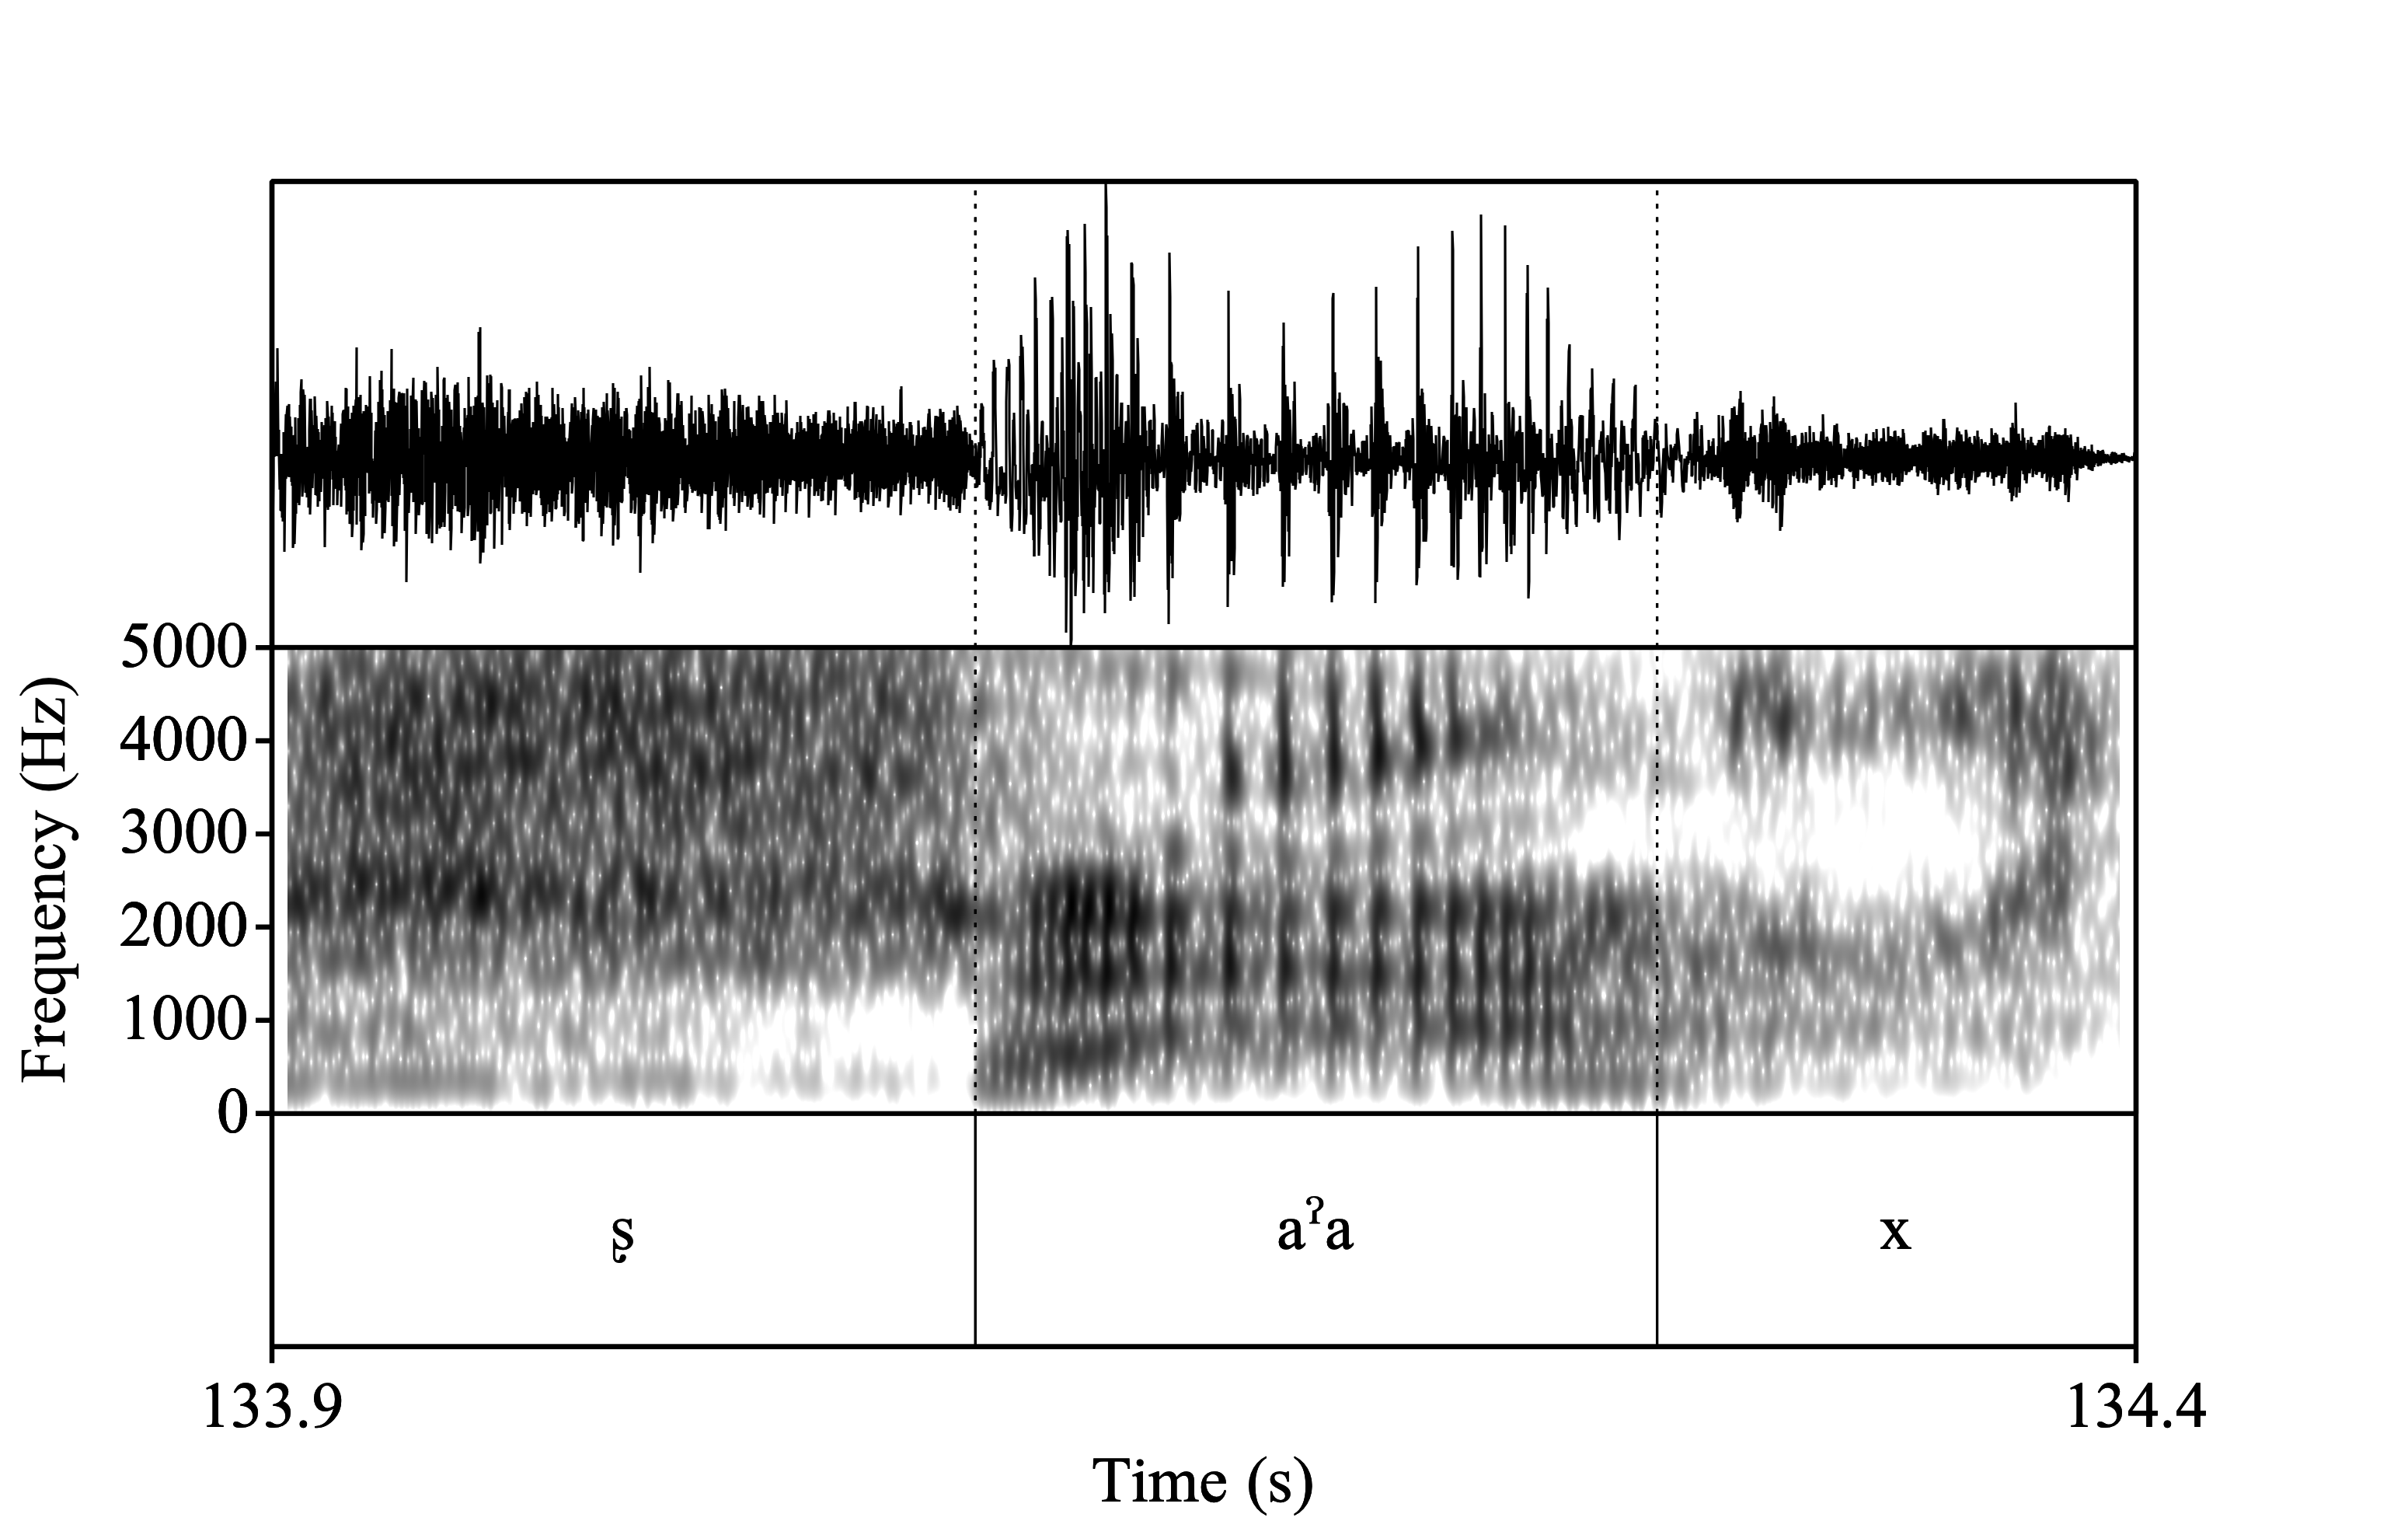
\includegraphics[width=\linewidth]{../xa'ag.png}
		\caption{\textit{xa'ag} `topil'}
		\label{fig:xa'ag}
	\end{subfigure}	
	\caption{Comparison of FSR's laryngealized vowels in \textit{za'a} `corncob' and \textit{xa'ag} `topil'}
	\label{fig:FSRLaryngeal}
\end{figure}

%------------------------------------
\subsection{Interaction of tone and phonation in Santiago Laxopa Zapotec} \label{sec:TonePhonation}
%------------------------------------

%------------------------------------
\section{Methodology} \label{sec:Methods}
%------------------------------------


%------------------------------------
\section{Results} \label{sec:Results}
%------------------------------------

%------------------------------------
\subsection{H1-H2 spectral-tilt} \label{}
%------------------------------------

%------------------------------------
\subsection{H1-A3 spectral-tilt} \label{}
%------------------------------------

%------------------------------------
\subsection{Cepstral Peak Prominence} \label{}
%------------------------------------

%------------------------------------
\section{Discussion} \label{sec:Discussion}
%------------------------------------

%------------------------------------
\subsection{Laryngeal Complexity Hypothesis} \label{}
%------------------------------------

\begin{itemize}
    \item \citet{silvermanLaryngealComplexityOtomanguean1997,blankenshipTimeCourseBreathiness1997,blankenshipTimingNonmodalPhonation2002}
\end{itemize}

%------------------------------------
%\subsection{} \label{}
%------------------------------------

%------------------------------------
\section{Conclusion} \label{sec:Conclusion}
%------------------------------------

%------------------------------------
%\subsection{} \label{}
%------------------------------------

%------------------------------------
%BIBLIOGRAPHY
%------------------------------------

%\singlespacing
% \nocite{*}
\printbibliography[heading=bibintoc]

\end{document} 